\chapter{Testes sintéticos para estimativa da direção de magnetização}
\label{chap:synt_tests}

Aplicamos o método proposto para estimar a direção de magnetização em três conjuntos de dados sintéticos simulando diferentes cenários geológicos. O primeiro deles é um modelo contendo um conjunto de fontes com diferentes geometrias e mesma direção de magnetização (Seção \ref{sec:unidir_model}). O segundo conjunto de dados é gerado por um modelo contendo múltiplas fontes com mesma direção de magnetização, porém uma delas representando uma fonte rasa (Seção \ref{sec:unidir_shallow}). No terceiro teste violamos a hipótese de magnetização unidirecional simulando uma fonte rasa com diferente direção de magnetização (Seção \ref{sec:difdir_shallow}).  

Em todos os testes, os dados simulados foram calculados em um grid regular de $49 \times 25$ pontos (um total de $N = 1225$ observações) a uma altura constante de $100$ m. Assumimos uma área de observação que se extende por $12$ km ao longo do eixo $x$ e do eixo $y$, resultando em um espaçamento entre os dados de $250$ m e $500$ m ao longo dos eixos $x$ e $y$, respectivamente. Os dados foram contaminados com um ruído Gaussiano de média zero e desvio padão de $10$ nT. O campo geomagnético principal simulado possui $I_0 = -40^\circ$ e $D_0 = -22^\circ$ para a inclinação e declinação, respectivamente. Para o processo de inversão, utilizamos uma camada equivalente composta por um grid de $49 \times 25$ dipolos (um total de $M = 1225$ fontes equivalentes) posicionados a uma profundidade de $z_c = 1150$ m abaixo do plano de observação ($2,5$ vezes o maior espaçamento entre os dados). Para a escolha do parâmetro de regularização ($\mu$) utilizamos a curva-L. Nosso algoritmo começa com uma aproximação inicial $\bar{\mathbf{q}}^{0} = (-10^\circ,-10^\circ)$ para a inclinação e a declinação, respectivamente. 

\section{Fontes de mesma direção de magnetização}
\label{sec:unidir_model}

Geramos um prisma poligonal cujo topo é posicionado a uma profundidade de $450$ m e a base a $3150$ m com intensidade de magnetização de $4$ A/m. Geramos também duas esferas com intensidade de magnetização igual a $3$ A/m e raio $500$ m. As coordenadas de seus respectivos centros são $x_c = 1800$ m, $y_c = -1800$ m e $z_c = 1000$ m e $x_c = 800$ m, $y_c = 800$ m and $z_c= 1000$ m. Simulamos dois prismas retangulares com $2.5$ A/m de intensidade de magnetização. O prisma menor possui topo a uma profundidade de $450$ m e lados de comprimento $1000$ m, $700$ m e $500$ m ao longo dos eixos $x$, $y$ e $z$, respectivamente. O prisma maior tem o topo localizado a uma profundidade de $500$ m e lados de comprimento $1000$ m, $2000$ m e $1550$ m ao longo dos eixos $x$, $y$ e $z$, respectivamente. Todas as fontes simuladas tem inclinação $-25^\circ$ e declinação $30^\circ$. O dado observado é mostrado na figura \ref{fig:data_fitting_1}a.

A figura \ref{fig:data_fitting_1}b mostra os dados preditos produzidos pela camada equivalente. A figura \ref{fig:data_fitting_1}c mostra os resíduos definidos pela diferença entre os dados simulados (Figura \ref{fig:data_fitting_1}a) e os dados preditos (Figura \ref{fig:data_fitting_1}b). Os resíduos aparecem com distribuição normal de média $-0,30 \, nT$ e desvio padrão $9,67 \, nT$ como mostrado na figura \ref{fig:data_fitting_1}d. A direção de magnetização estimada $\bar{\mathbf{q}}$ tem inclinação $-28,6^\circ$ e declinação $30,8^\circ$, que são muito próximas a direção verdadeira. A distribuição de momentos magnéticos positivos $\bar{\mathbf{p}}$ é mostrada na figura \ref{fig:dist_momentos_pos_1}. A convergência do algoritmo é mostrado na figura \ref{fig:convergence_1}. Consideramos que o método foi bem sucedido em estimar a direção de magnetização das múltiplas fontes do modelo, de forma que a distribuição de momentos magnéticos produziu um bom ajuste dos dados observados. 

%%% Figuras teste 1 
\begin{figure}
	\centering
	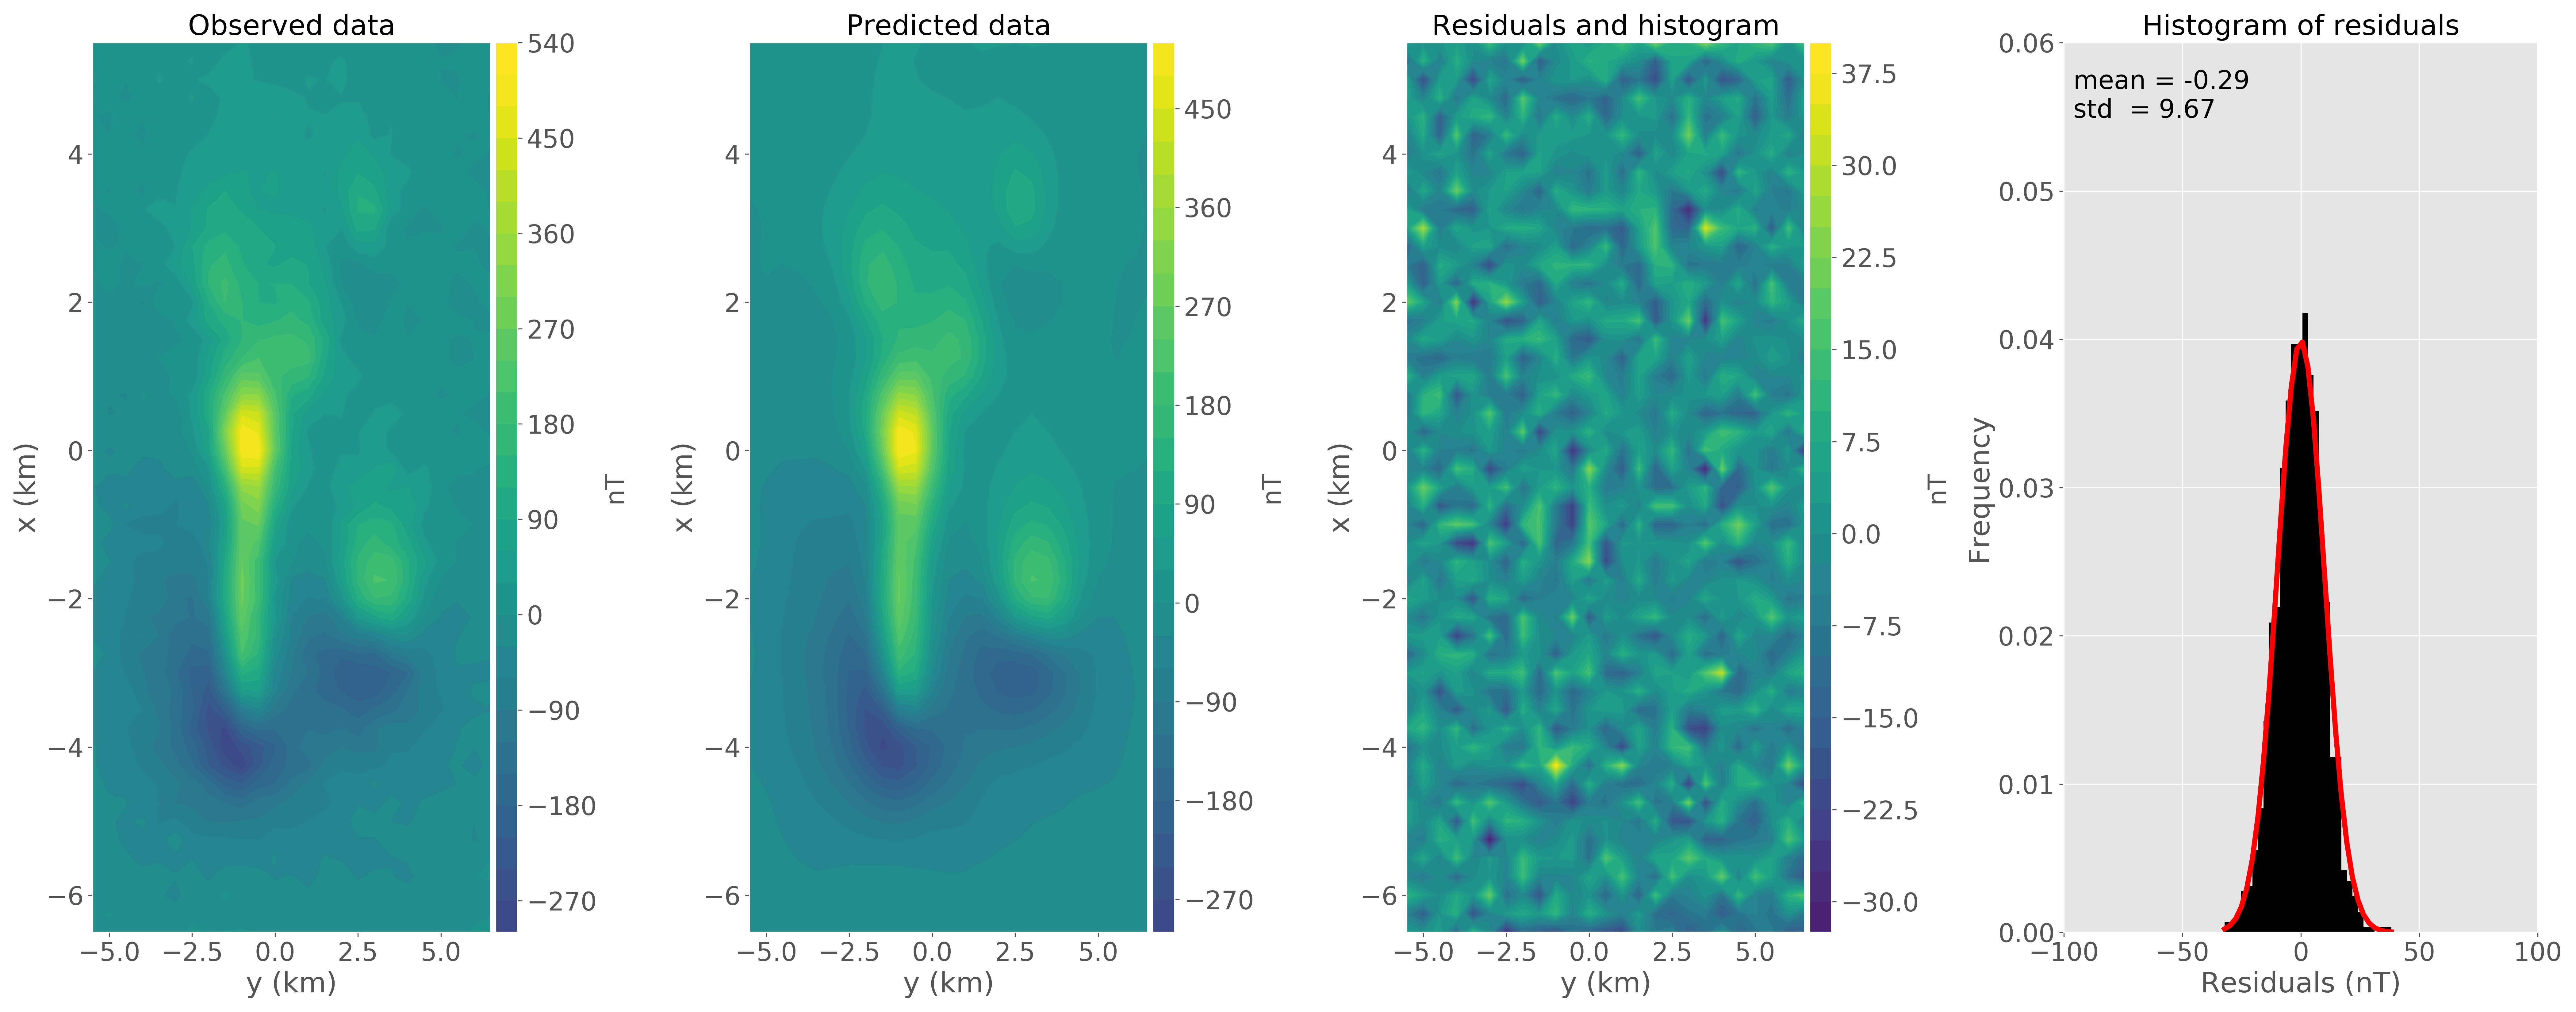
\includegraphics[width=1.1\textwidth]{Fig/eqlayer/unidir_test/data_fitting_LM_NNLS_magRM.png}
	\caption{Aplicação a dados sintéticos para múltiplas fontes com a mesma direção de magnetização. (a) Anomalia de campo total observada. (b) Dados preditos produzido pela camada equivalente. (c) Diferença entre os dados mostrados nos gráficos a e b. (d) Histograma dos resíduos.}
	\label{fig:data_fitting_1}
\end{figure}

\begin{figure}
	\centering
	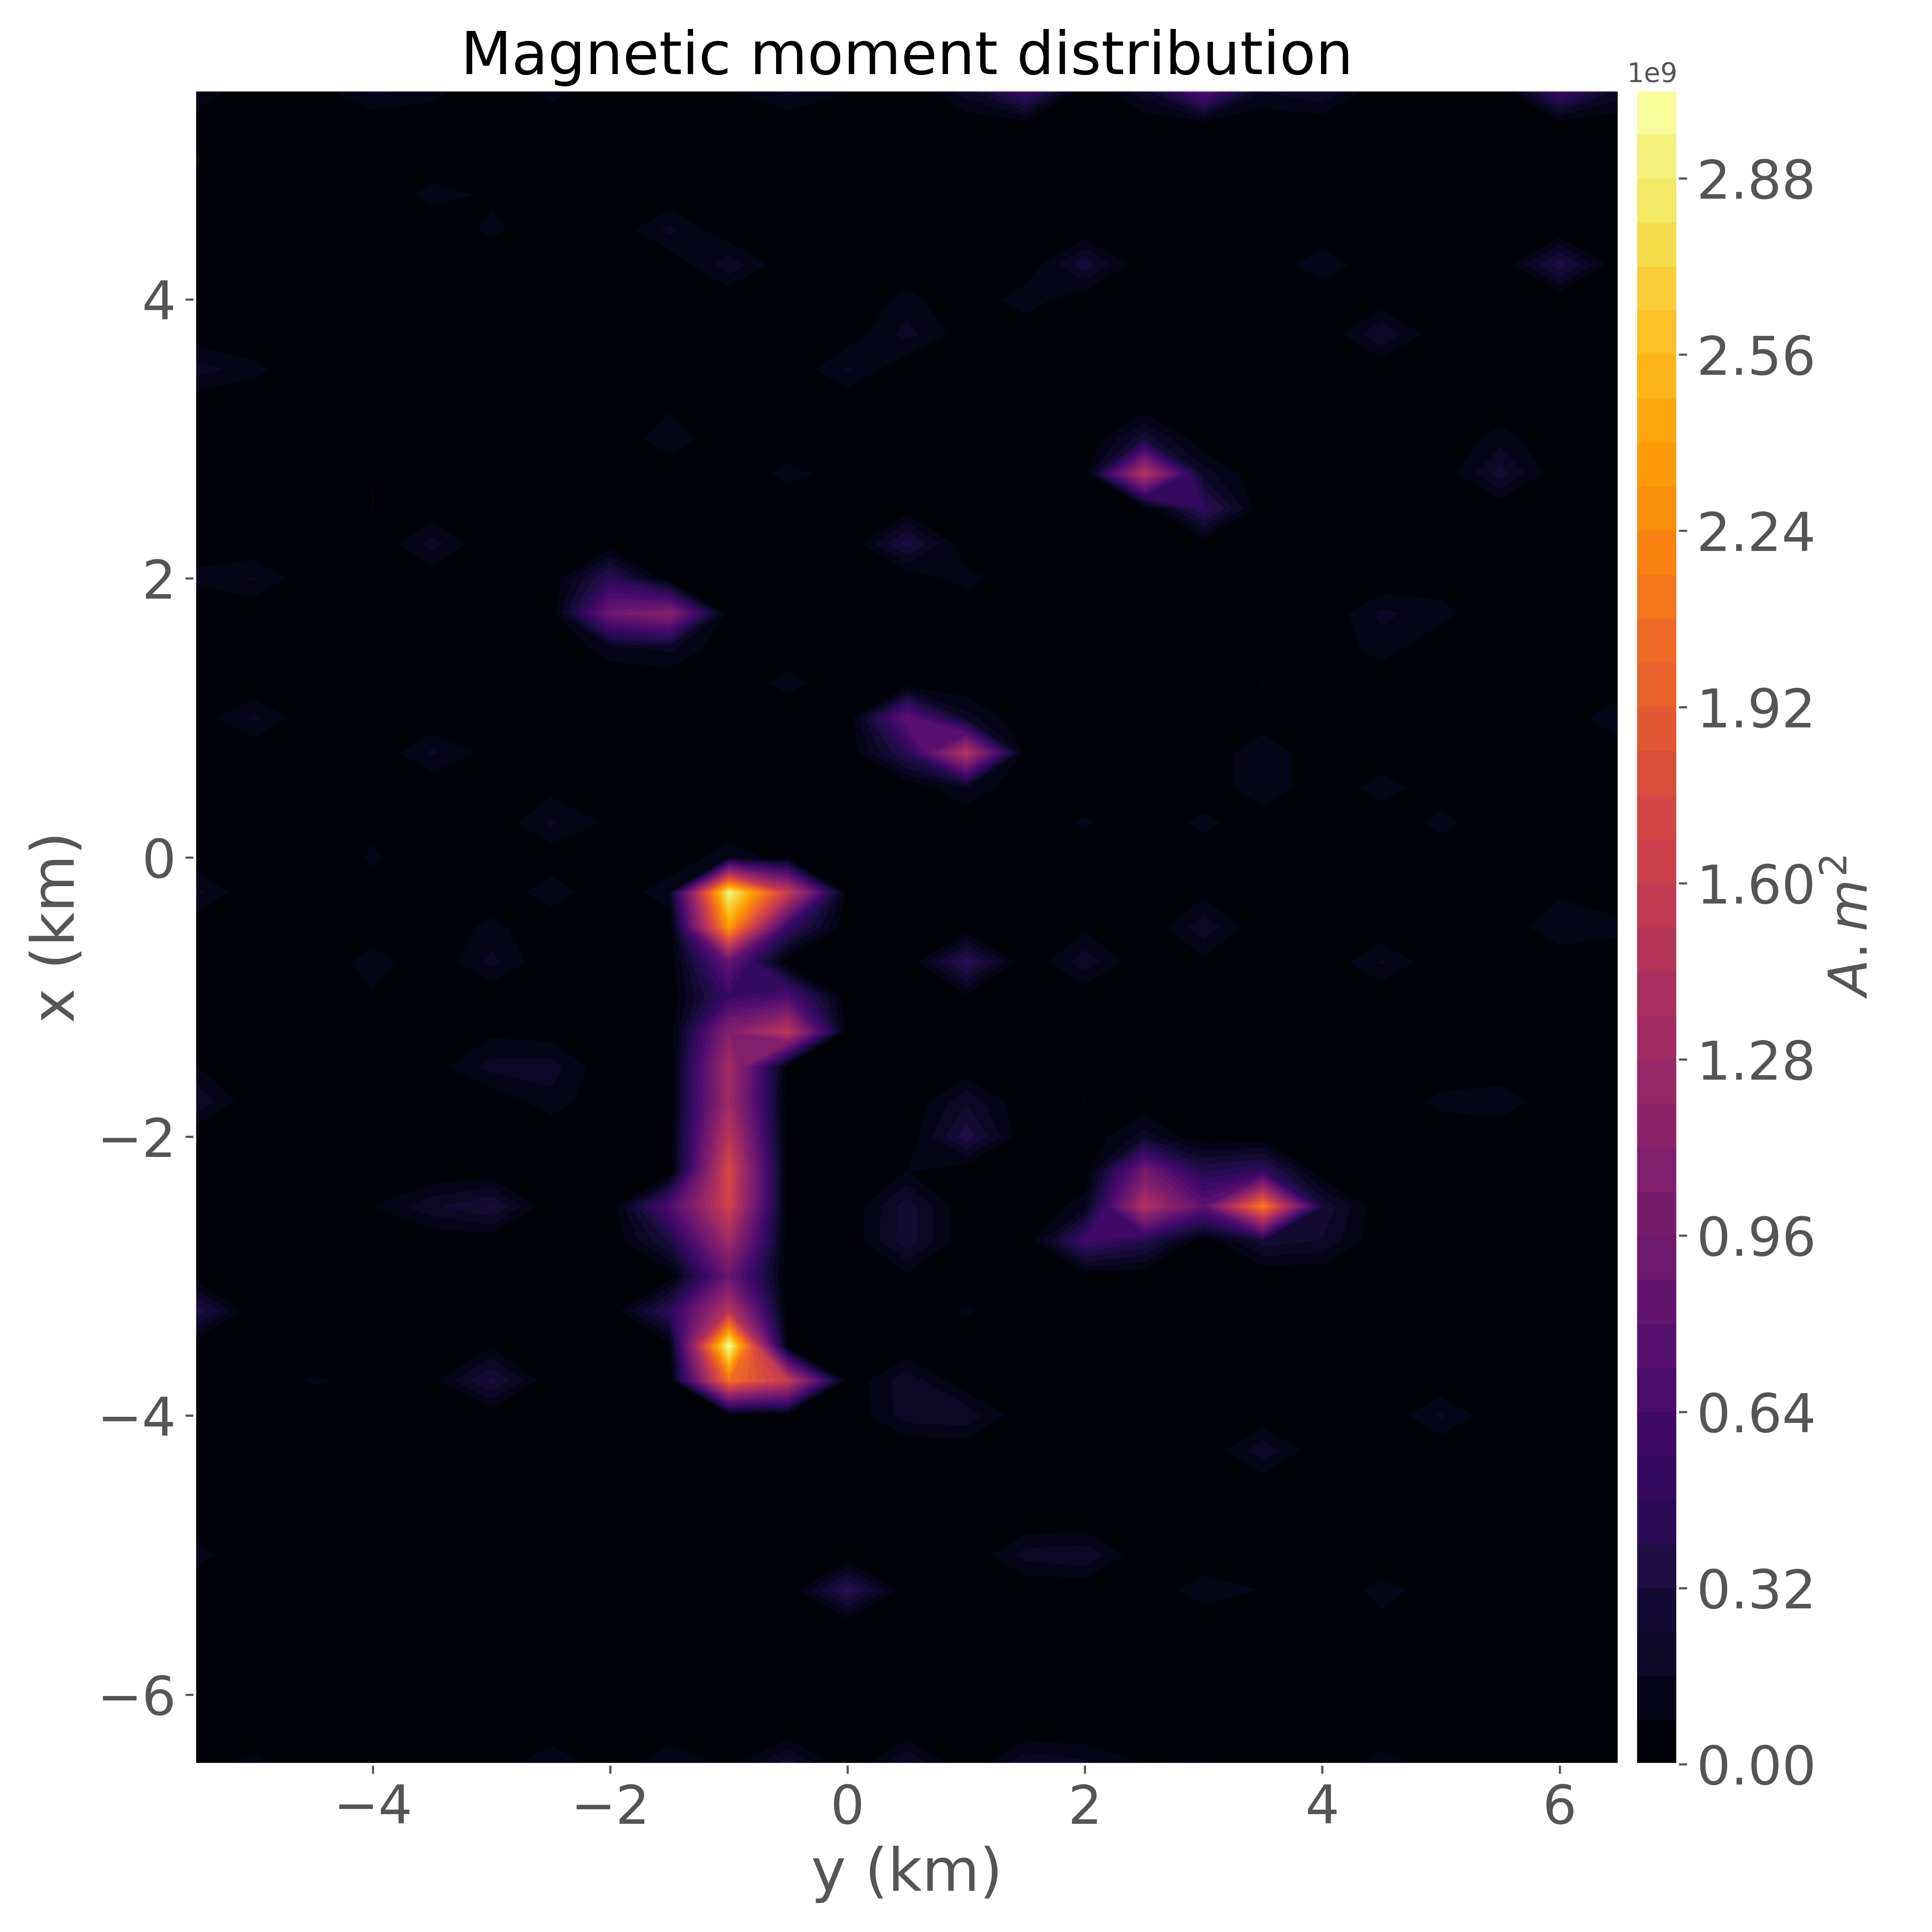
\includegraphics[width=.9\textwidth]{Fig/eqlayer/unidir_test/magnetic_moment_positive_LM_NNLS_magRM.png}
	\caption{Distribuição de momentos magnéticos positiva para a aplicação a dados sintéticos para múltiplas fontes de mesma direção de magnetização.}
	\label{fig:dist_momentos_pos_1}
\end{figure}

\begin{figure}
	\centering
	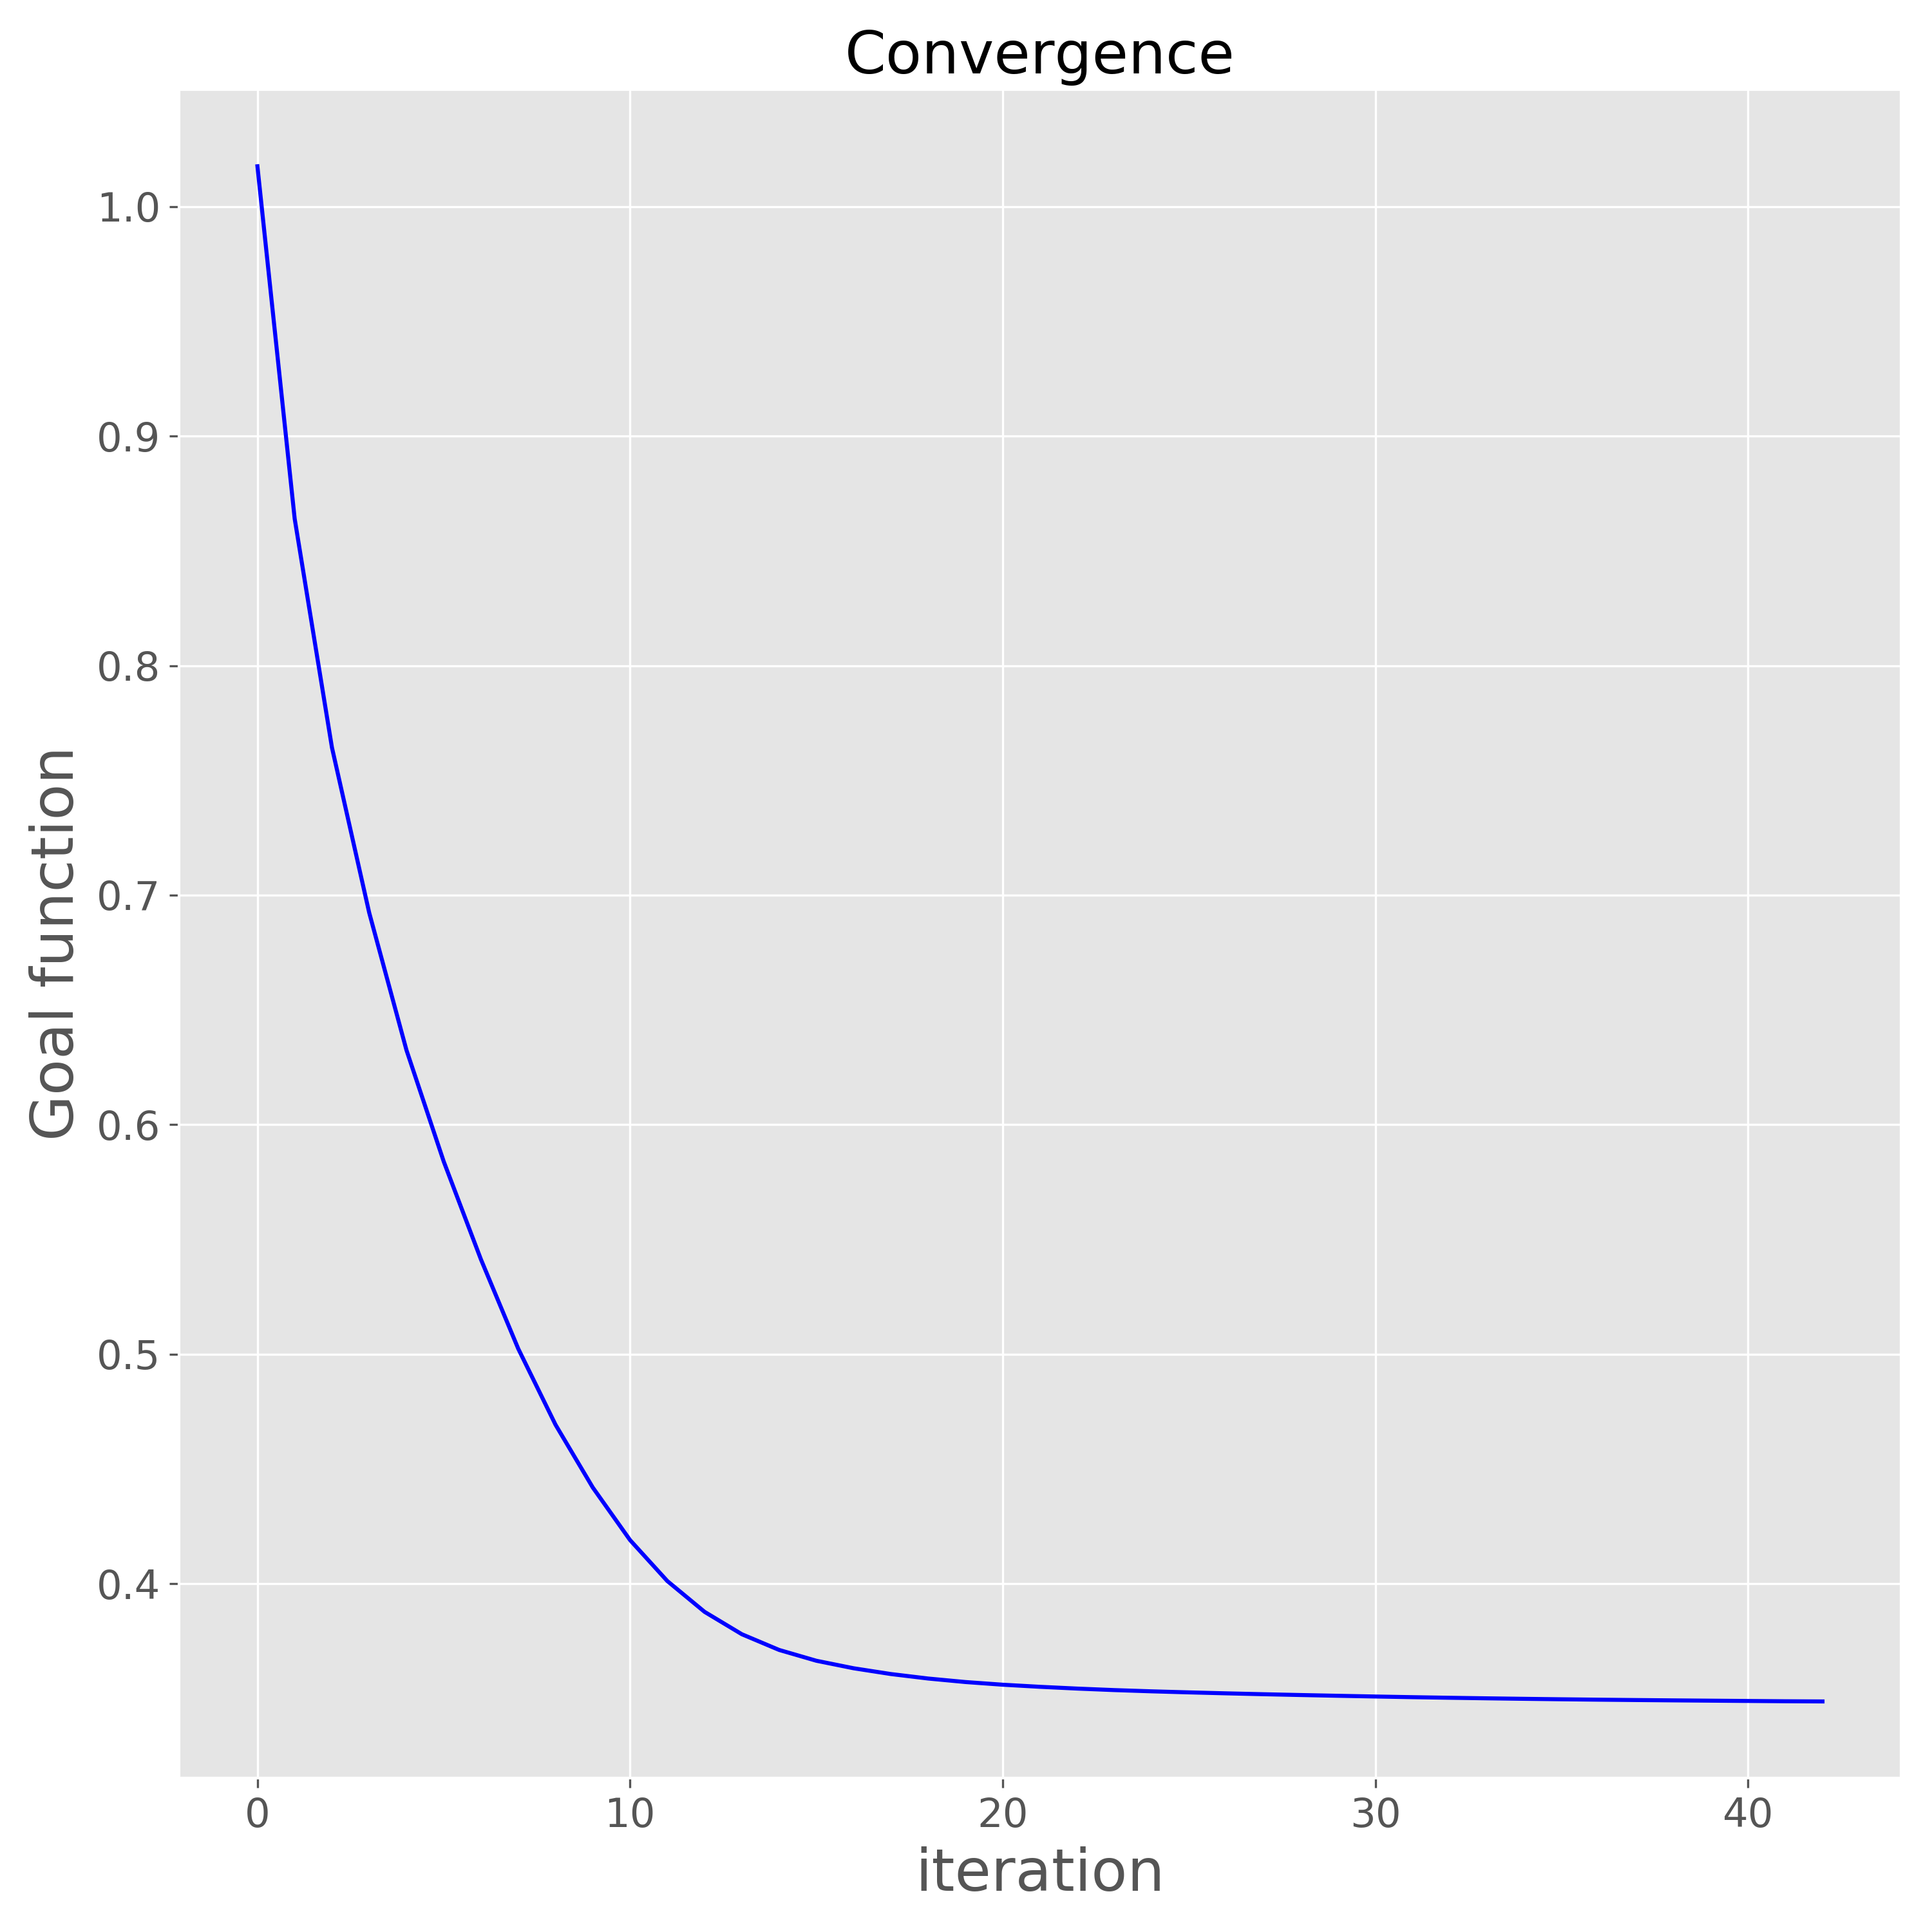
\includegraphics[width=.9\textwidth]{Fig/eqlayer/unidir_test/convergence_LM_NNLS_magRM.png}
	\caption{Valor da função objetivo ao longo das iterações (equação \ref{eq:positivity_goal_function}a) mostrando a convergência do algoritmo.}
	\label{fig:convergence_1}
\end{figure}


\section{Magnetização unidirecional com fonte rasa}
\label{sec:unidir_shallow}

Testamos a performance do método quando existe uma fonte rasa. O modelo é similar ao anterior com exceção do prisma menor, cujo topo é localizado a uma profundidade de $150$ m enquanto seu volume é mantido o mesmo. A intensidade de magnetização deste prisma raso é igual a $1,5$ A/m. A direção de magnetização de todas as fontes é $-25^\circ$ de inclinação e $30^\circ$ graus para a declinação. Os dados sintéticos são mostrados na figura \ref{fig:data_fitting_2}a.

A figura \ref{fig:data_fitting_2}b mostra a anomalia de campo total predita produzida pela camada equivalente. A figura \ref{fig:data_fitting_2}c mostra o mapa dos resíduos definido como a diferença entre a anomalia de campo total observada (Figura \ref{fig:data_fitting_2}a) e a anomalia de campo total predita (Figura \ref{fig:data_fitting_2}b). Os resíduos aparecem com uma distribuição normal de média $-0,42$ nT e desvio padrão de $10,67$ nT como mostra a figura \ref{fig:data_fitting_2}d. A figura \ref{fig:dist_momentos_pos_2} mostra a distribuição de momentos magnéticos $\bar{\mathbf{p}}$. A convergência do algoritmo é mostrada na figura \ref{fig:convergence_2}. Apesar do grande resíduo acima da fonte rasa, consideramos que a metodologia produziu uma confiável estimativa para a direção de magnetização $\bar{\mathbf{q}}$, que possui inclinação $-28,7^\circ$ e declination $31,7^\circ$. A direção de magnetização estimada é próxima a direção verdadeira e a distribuição de momentos magnéticos produziu um ajuste aceitável dos dados. 

%%% Figuras teste 2 
\begin{figure}
	\centering
	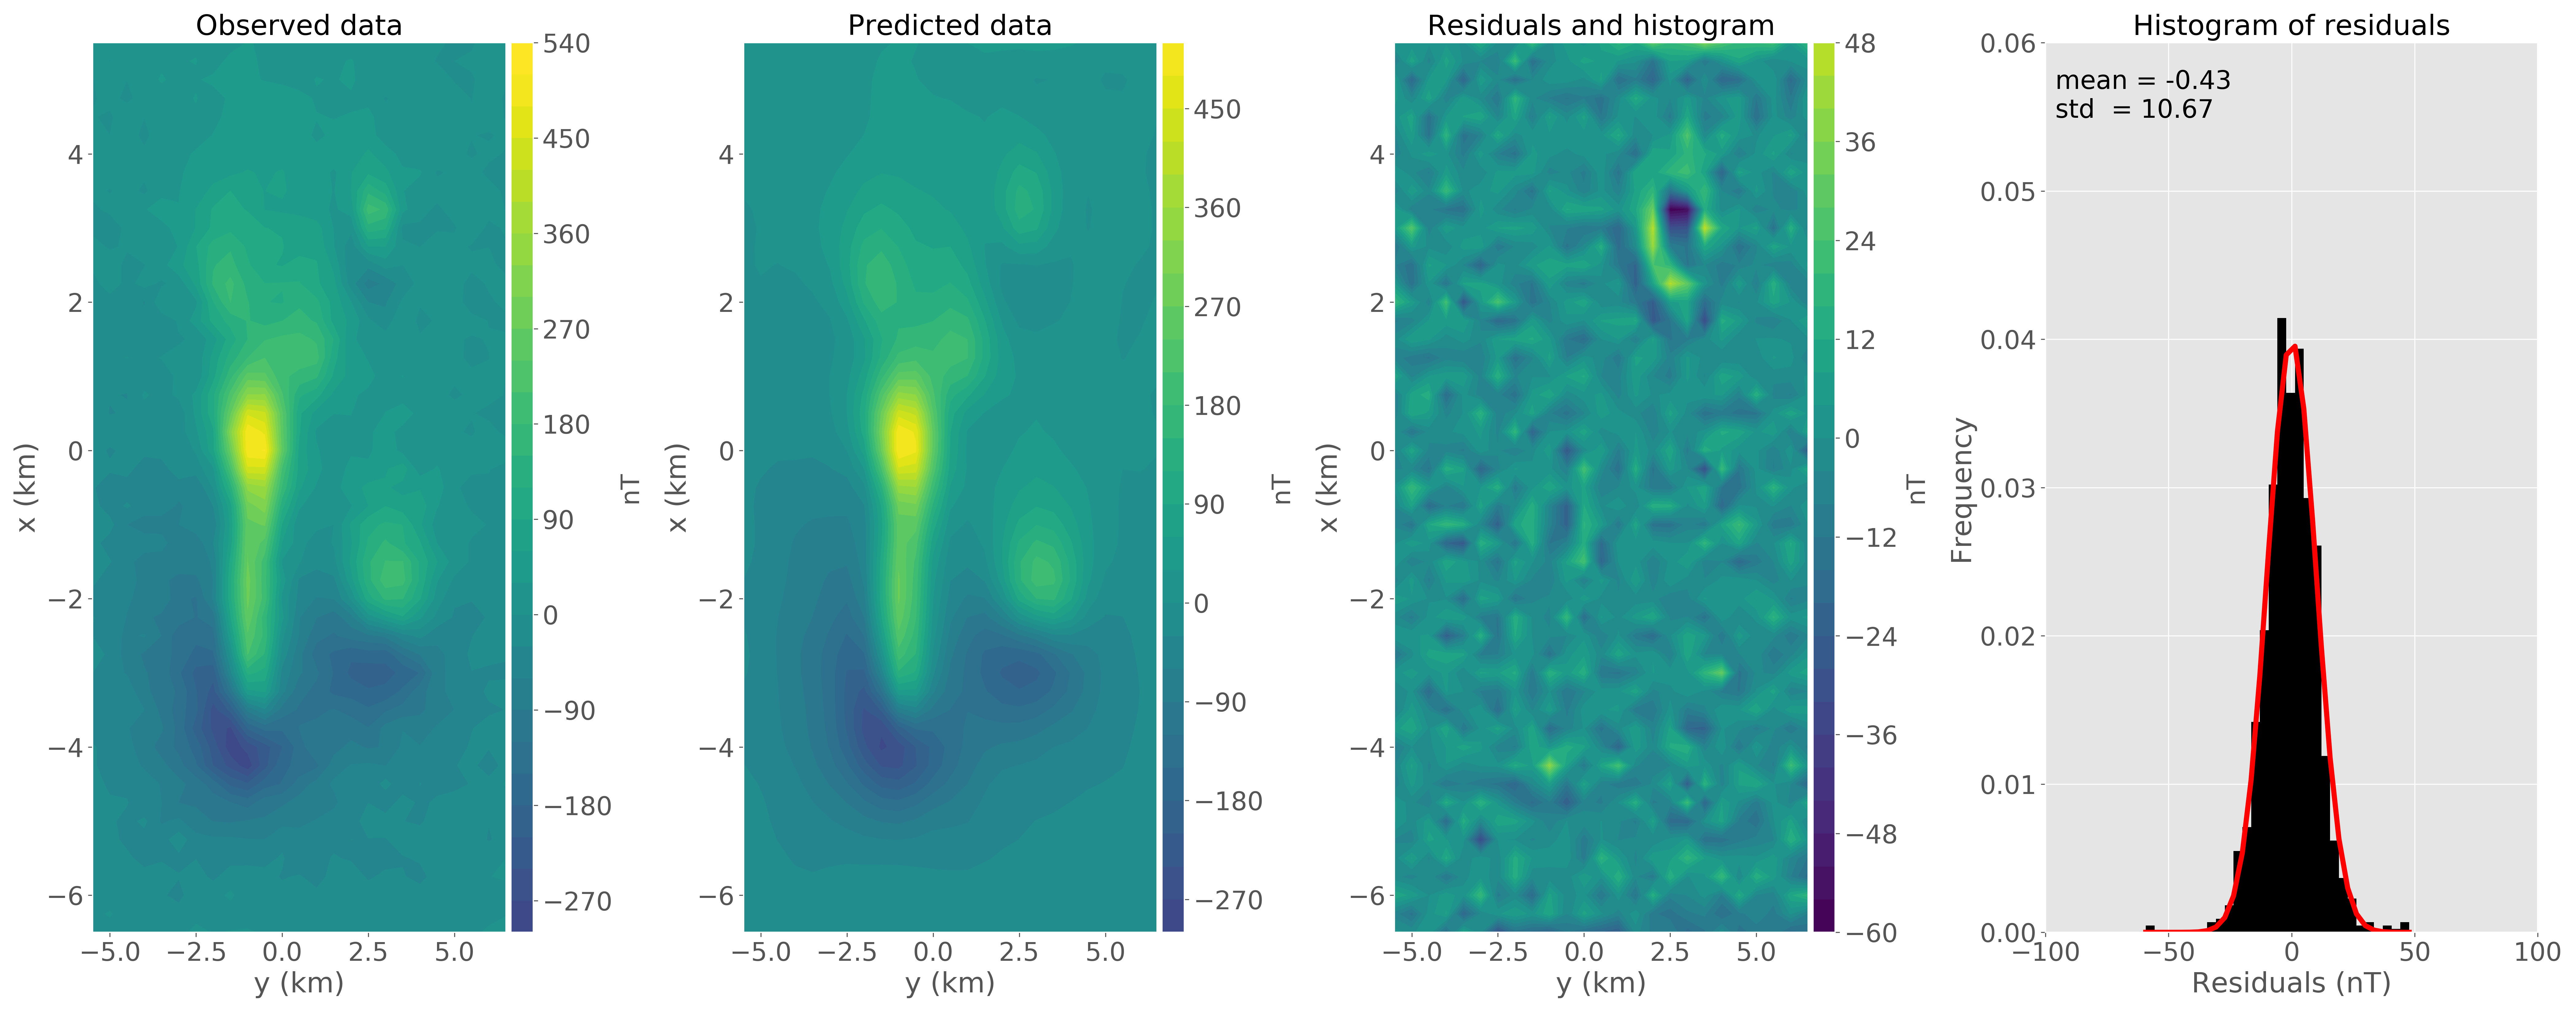
\includegraphics[width=1.1\textwidth]{Fig/eqlayer/unidir_shallow_test/data_fitting_LM_NNLS_magRM.png}
	\caption{Aplicação a dados sintéticos para múltiplos corpos com uma fonte rasa e mesma direção de magnetização. (a) Anomalia de campo total observada. (b) Dados preditos produzido pela camada equivalente. (c) Diferença entre os dados mostrados nos gráficos a e b. (d) Histograma dos resíduos.}
	\label{fig:data_fitting_2}
\end{figure}

\begin{figure}
	\centering
	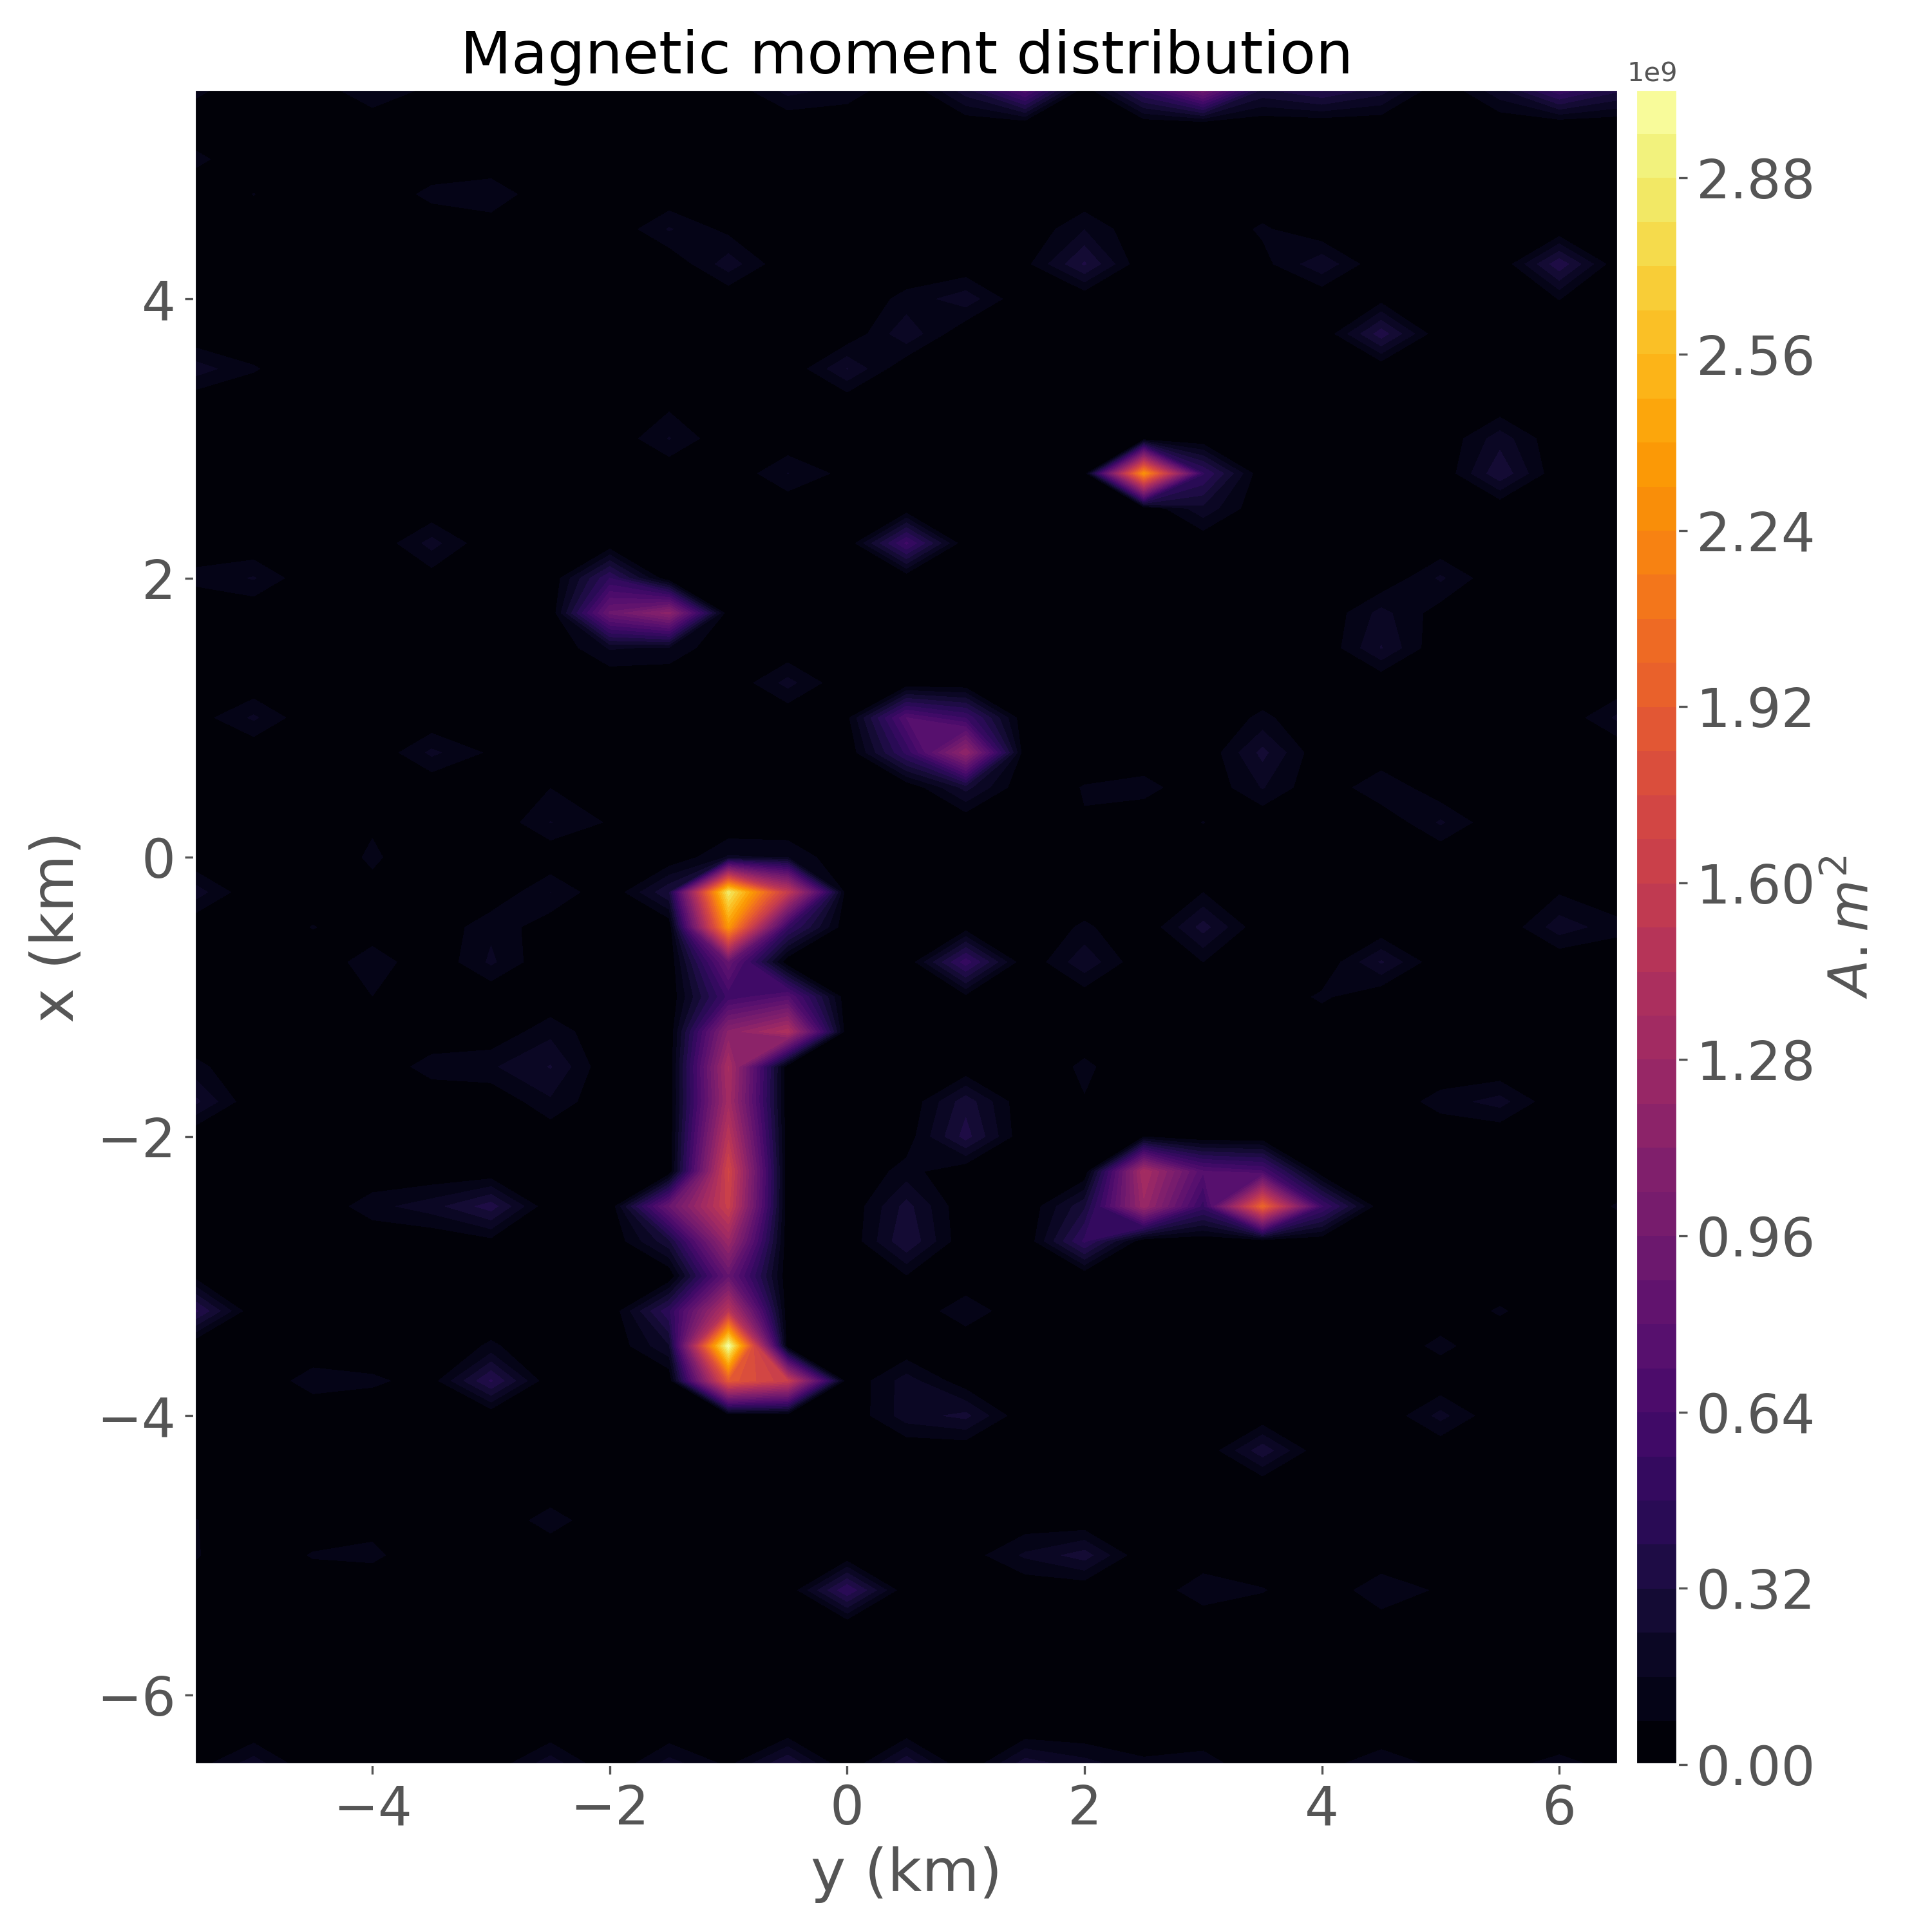
\includegraphics[width=.9\textwidth]{Fig/eqlayer/unidir_shallow_test/magnetic_moment_positive_LM_NNLS_magRM.png}
	\caption{Distribuição de momentos magnéticos positiva para a aplicação a dados sintéticos para múltiplos corpos e uma fonte rasa com mesma direção de magnetização.}
	\label{fig:dist_momentos_pos_2}
\end{figure}

\begin{figure}
	\centering
	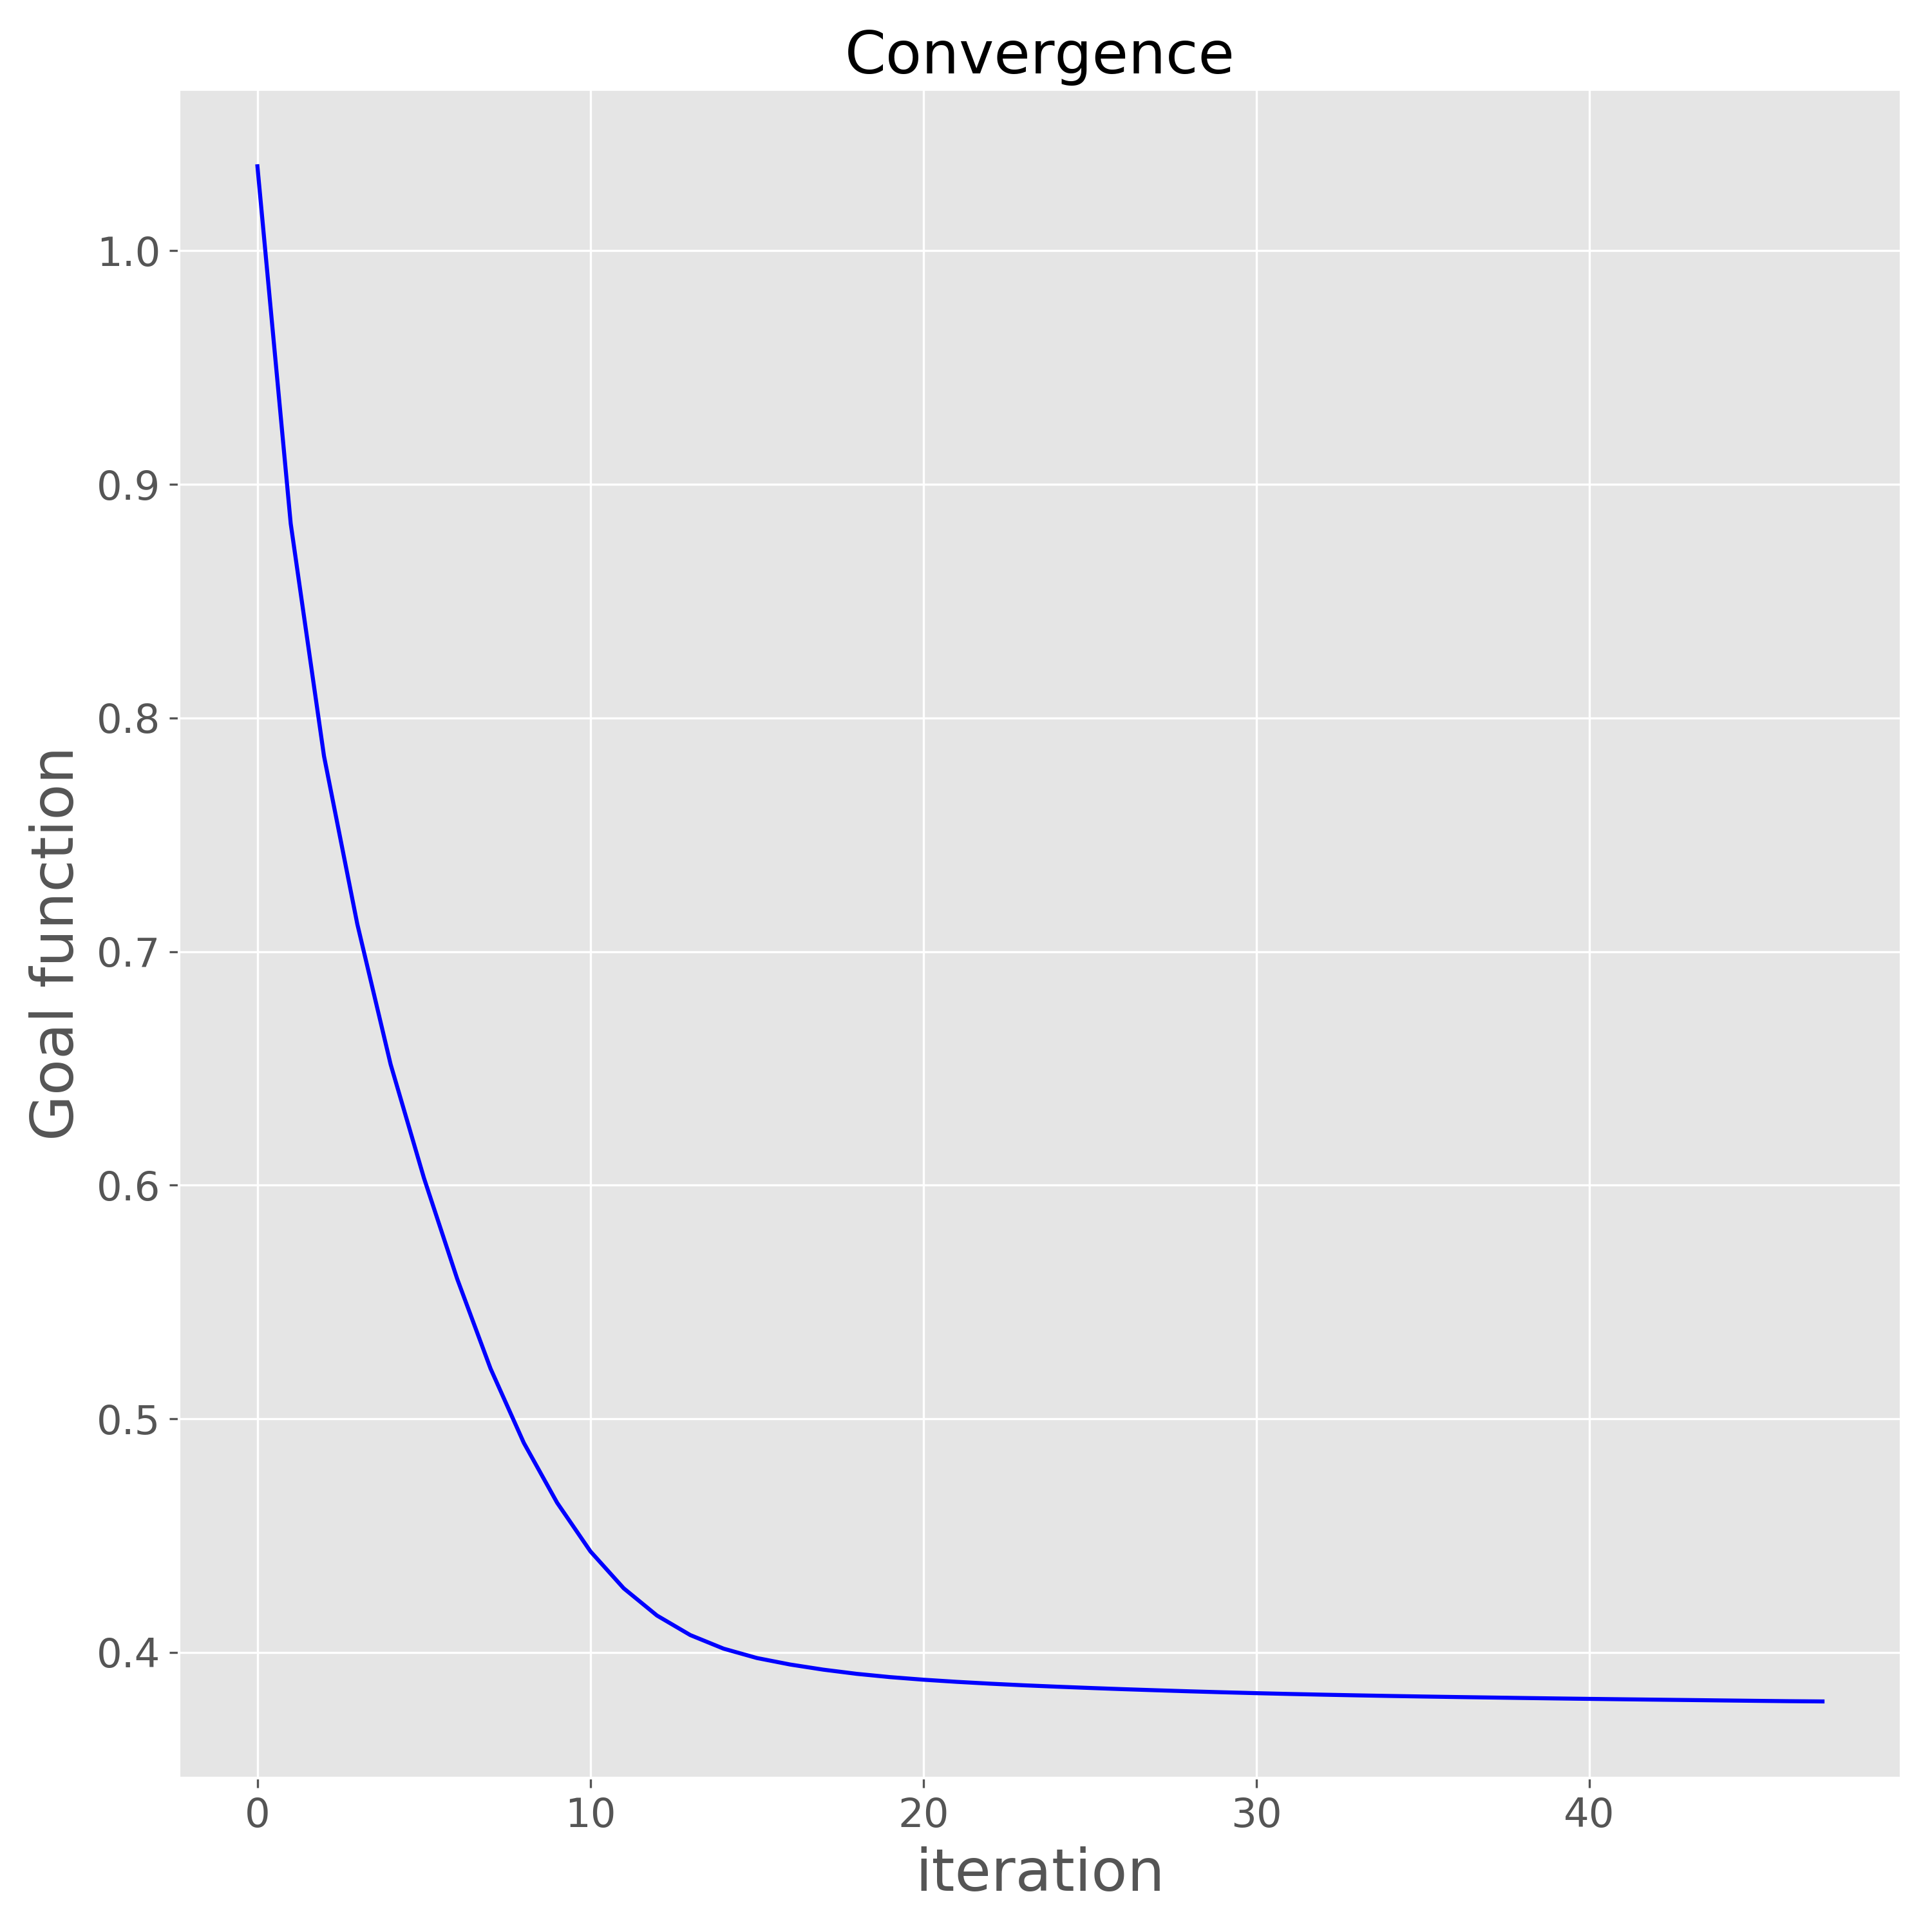
\includegraphics[width=.9\textwidth]{Fig/eqlayer/unidir_shallow_test/convergence_LM_NNLS_magRM.png}
	\caption{Valor da função objetivo ao longo das iterações (equação \ref{eq:positivity_goal_function}a) mostrando a convergência do algoritmo.}
	\label{fig:convergence_2}
\end{figure}

\section{Fonte rasa com direção de magnetização diferente}
\label{sec:difdir_shallow}

Neste teste simulamos a presença de uma fonte rasa com direção de magnetização diferente das demais. O prisma raso tem dimensão igual ao do teste anterior. No entanto, a direção de magnetização deste prisma é $20^\circ$ de inclinação e $-30^\circ$ de declinação, enquanto as outras fontes possuem inclinação $-25^\circ$ e declinação $30^\circ$. Os dados calculados são mostrados na figura \ref{fig:data_fitting_3}a. 

A figura \ref{fig:data_fitting_3}b mostra a anomalia de campo total predita pela camada equivalente. O mapa dos resíduos é mostrado na figura \ref{fig:data_fitting_3}c, e é definido como a diferença entre os dados observados (Figura \ref{fig:data_fitting_3}a) e os dados preditos (Figura \ref{fig:data_fitting_3}b). Os resíduos tem média igual a $-0,73$ nT e desvio padrão igual a  $12,67$ nT como mostra a figura \ref{fig:data_fitting_3}d. A direção de magnetização estimada $\bar{\mathbf{q}}$ tem inclinação $-30,4^\circ$ e declinação $27,6^\circ$. A figura \ref{fig:dist_momentos_pos_3} mostra a distribuição de momentos magnéticos positiva. A convergência do algoritmo é mostrada na figura \ref{fig:convergence_3}. Apesar da diferença em relação a direção de magnetização verdadeira, a distribuição de momentos positiva produziu um ajuste aceitável dos dados observados. Com exceção da pequena área acima da fonte rasa, a maior parte dos resíduos são próximos de $0$ nT. 

%%% Figuras teste 3
\begin{figure}
	\centering
	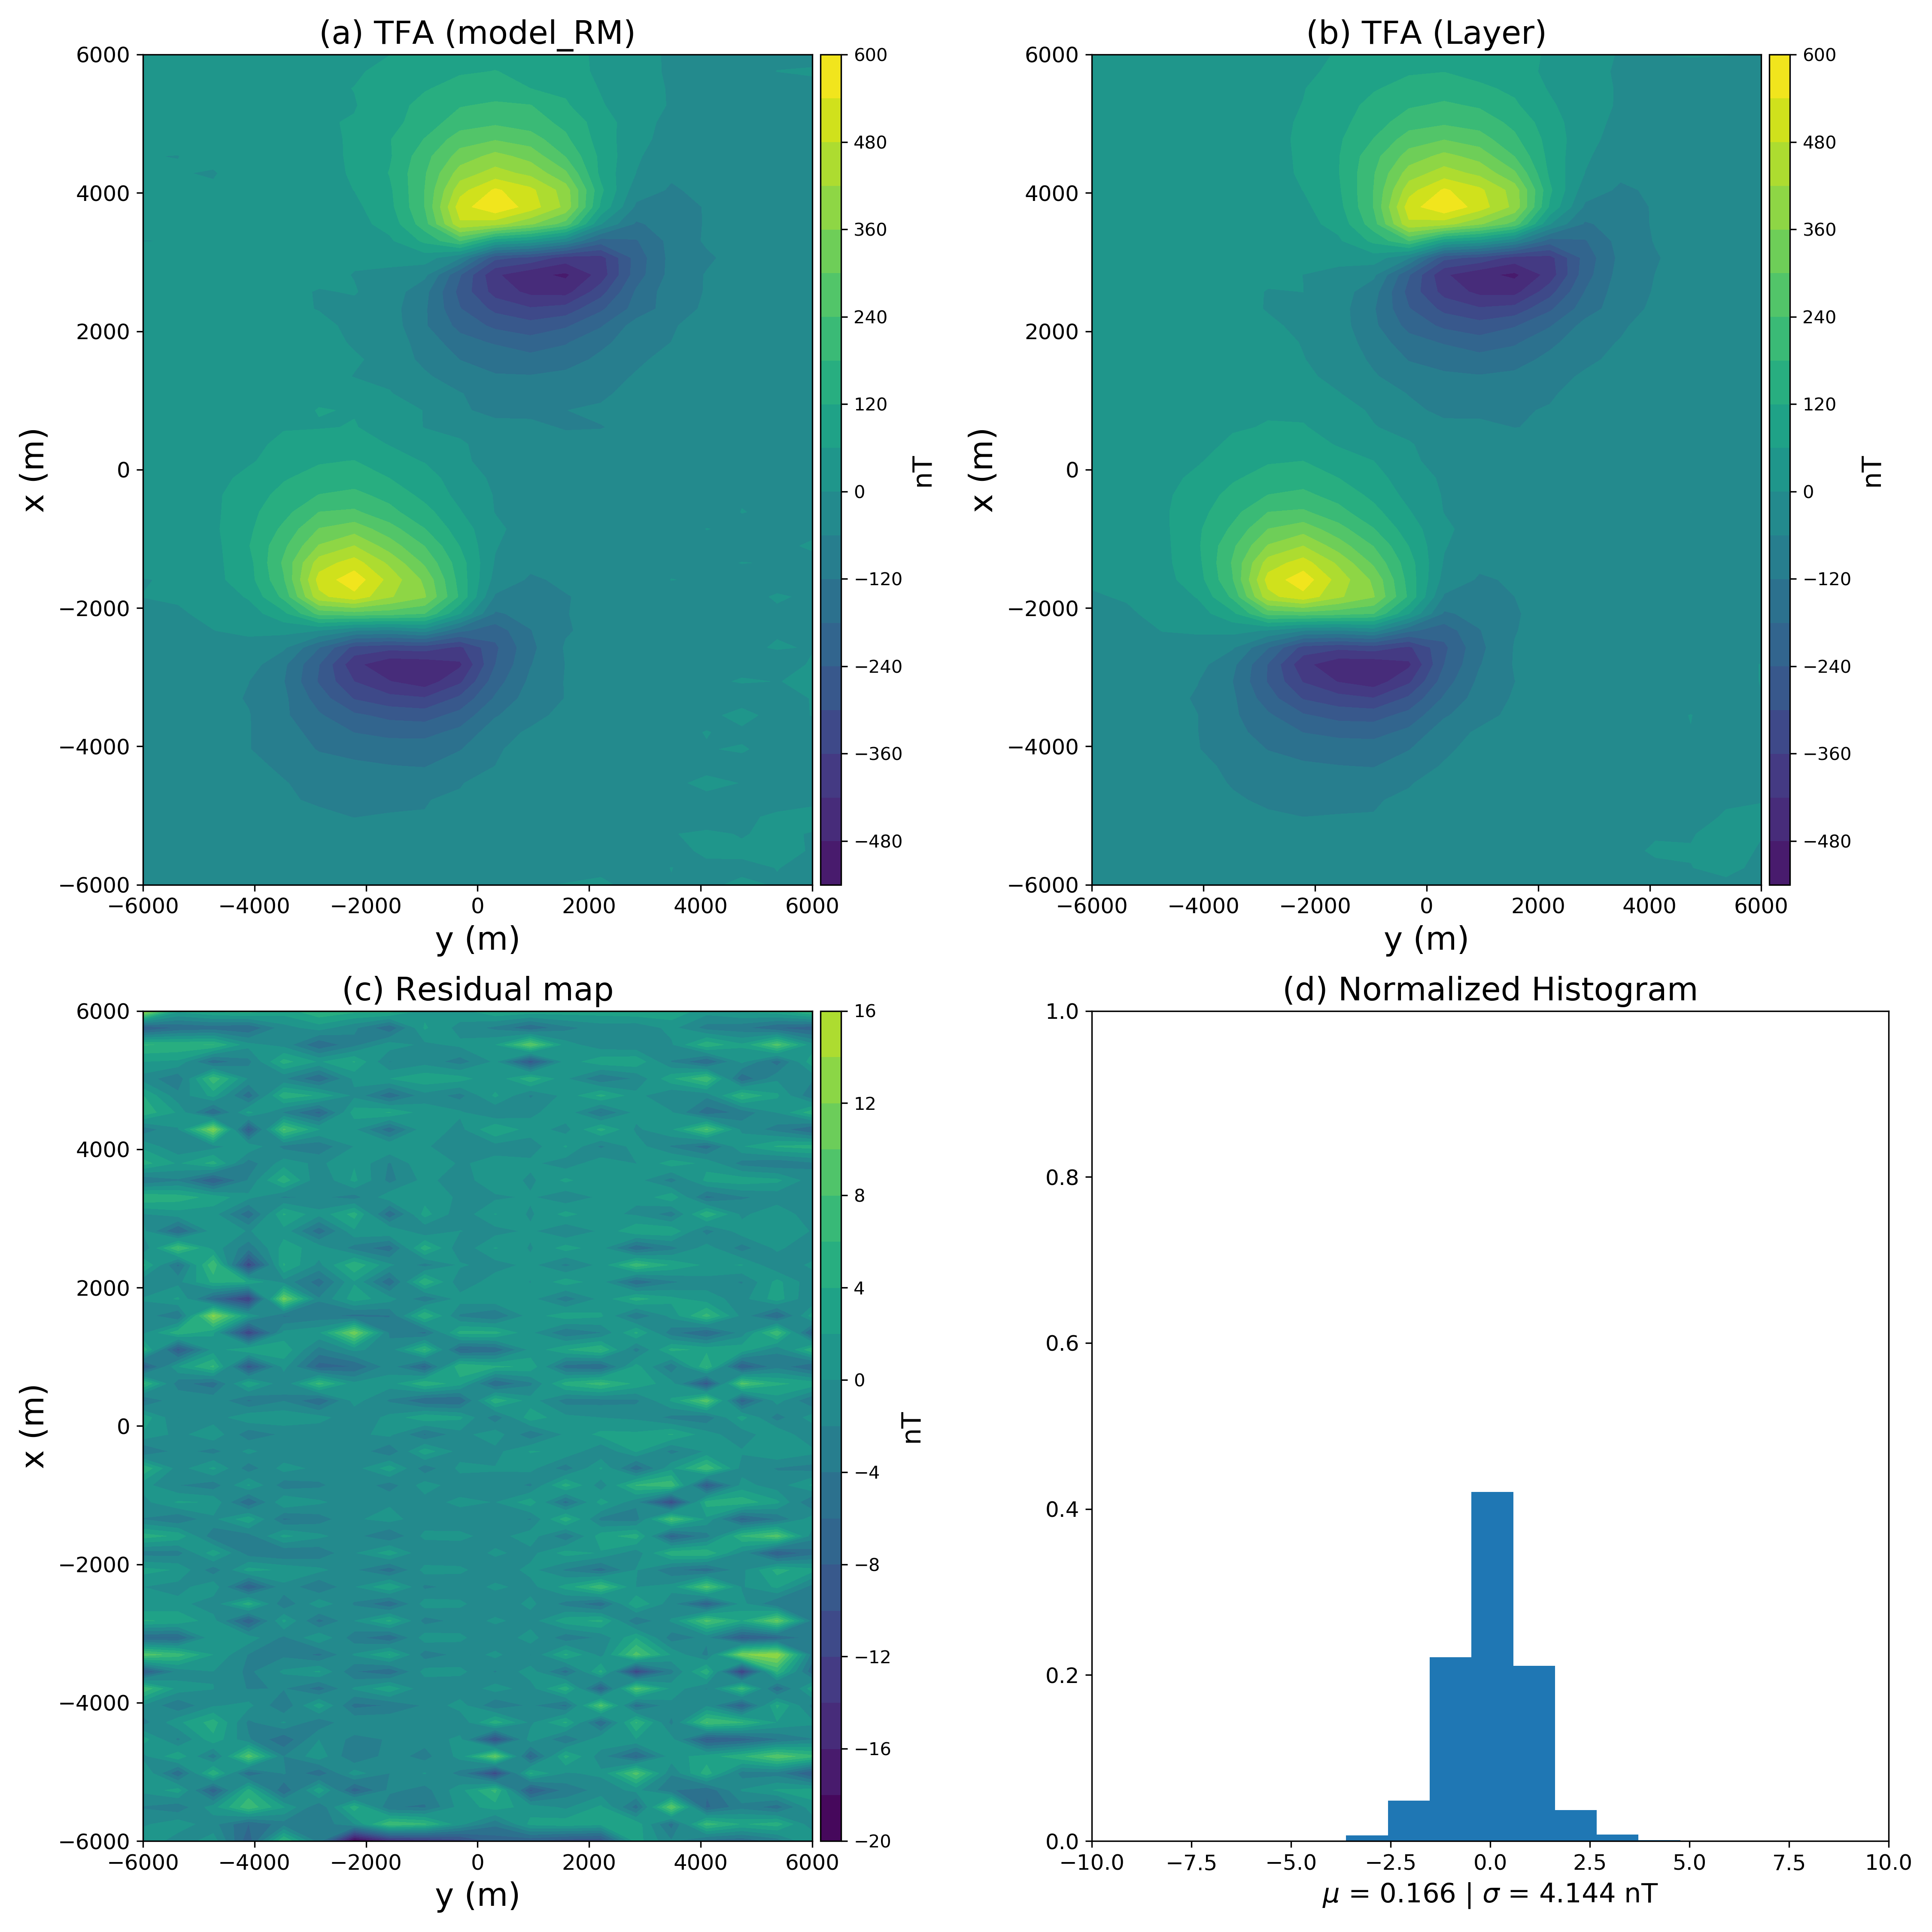
\includegraphics[width=1.1\textwidth]{Fig/eqlayer/unidir_shallow_diff_test/data_fitting_LM_NNLS_magRM.png}
	\caption{Aplicação a dados sintéticos para fonte rasa com direção de magnetização diferente. (a) Anomalia de campo total observada. (b) Dados preditos produzido pela camada equivalente. (c) Diferença entre os dados mostrados nos gráficos a e b. (d) Histograma dos resíduos.}
	\label{fig:data_fitting_3}
\end{figure}

\begin{figure}
	\centering
	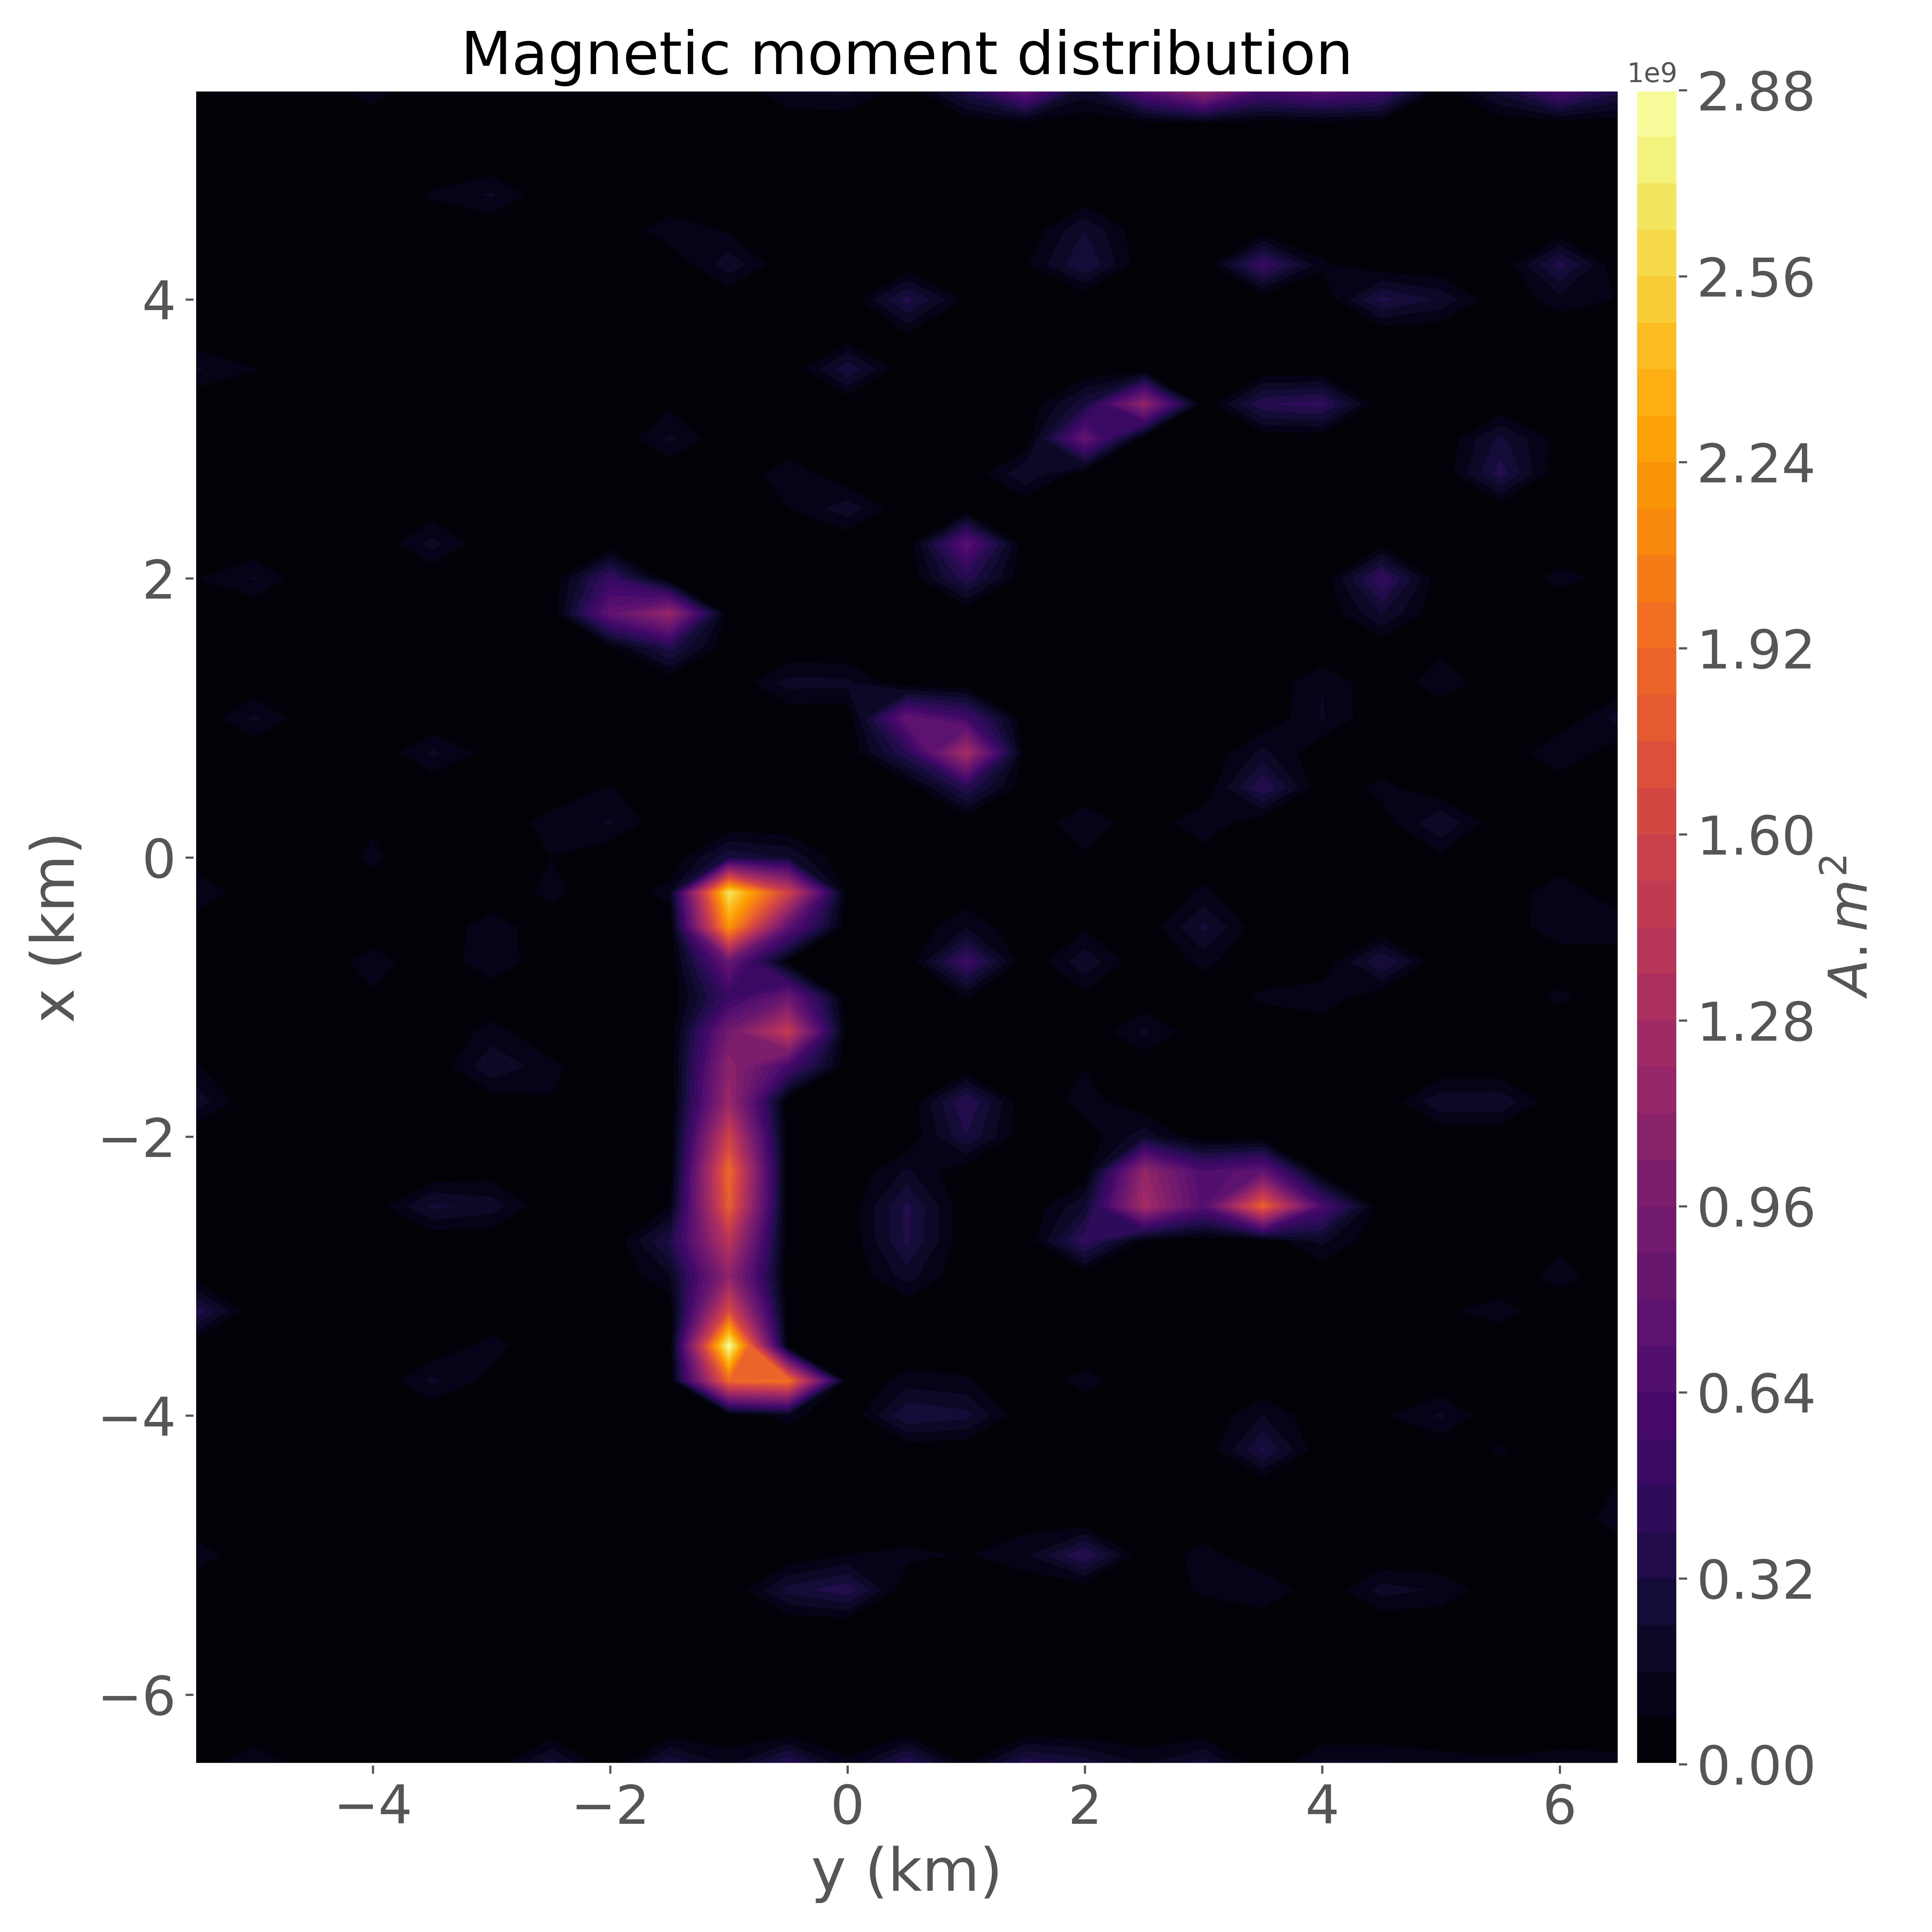
\includegraphics[width=.9\textwidth]{Fig/eqlayer/unidir_shallow_diff_test/magnetic_moment_positive_LM_NNLS_magRM.png}
	\caption{Distribuição de momentos magnéticos positiva para a aplicação a dados sintéticos para múltiplos corpos e uma fonte rasa com direção de magnetização diferente.}
	\label{fig:dist_momentos_pos_3}
\end{figure}

\begin{figure}
	\centering
	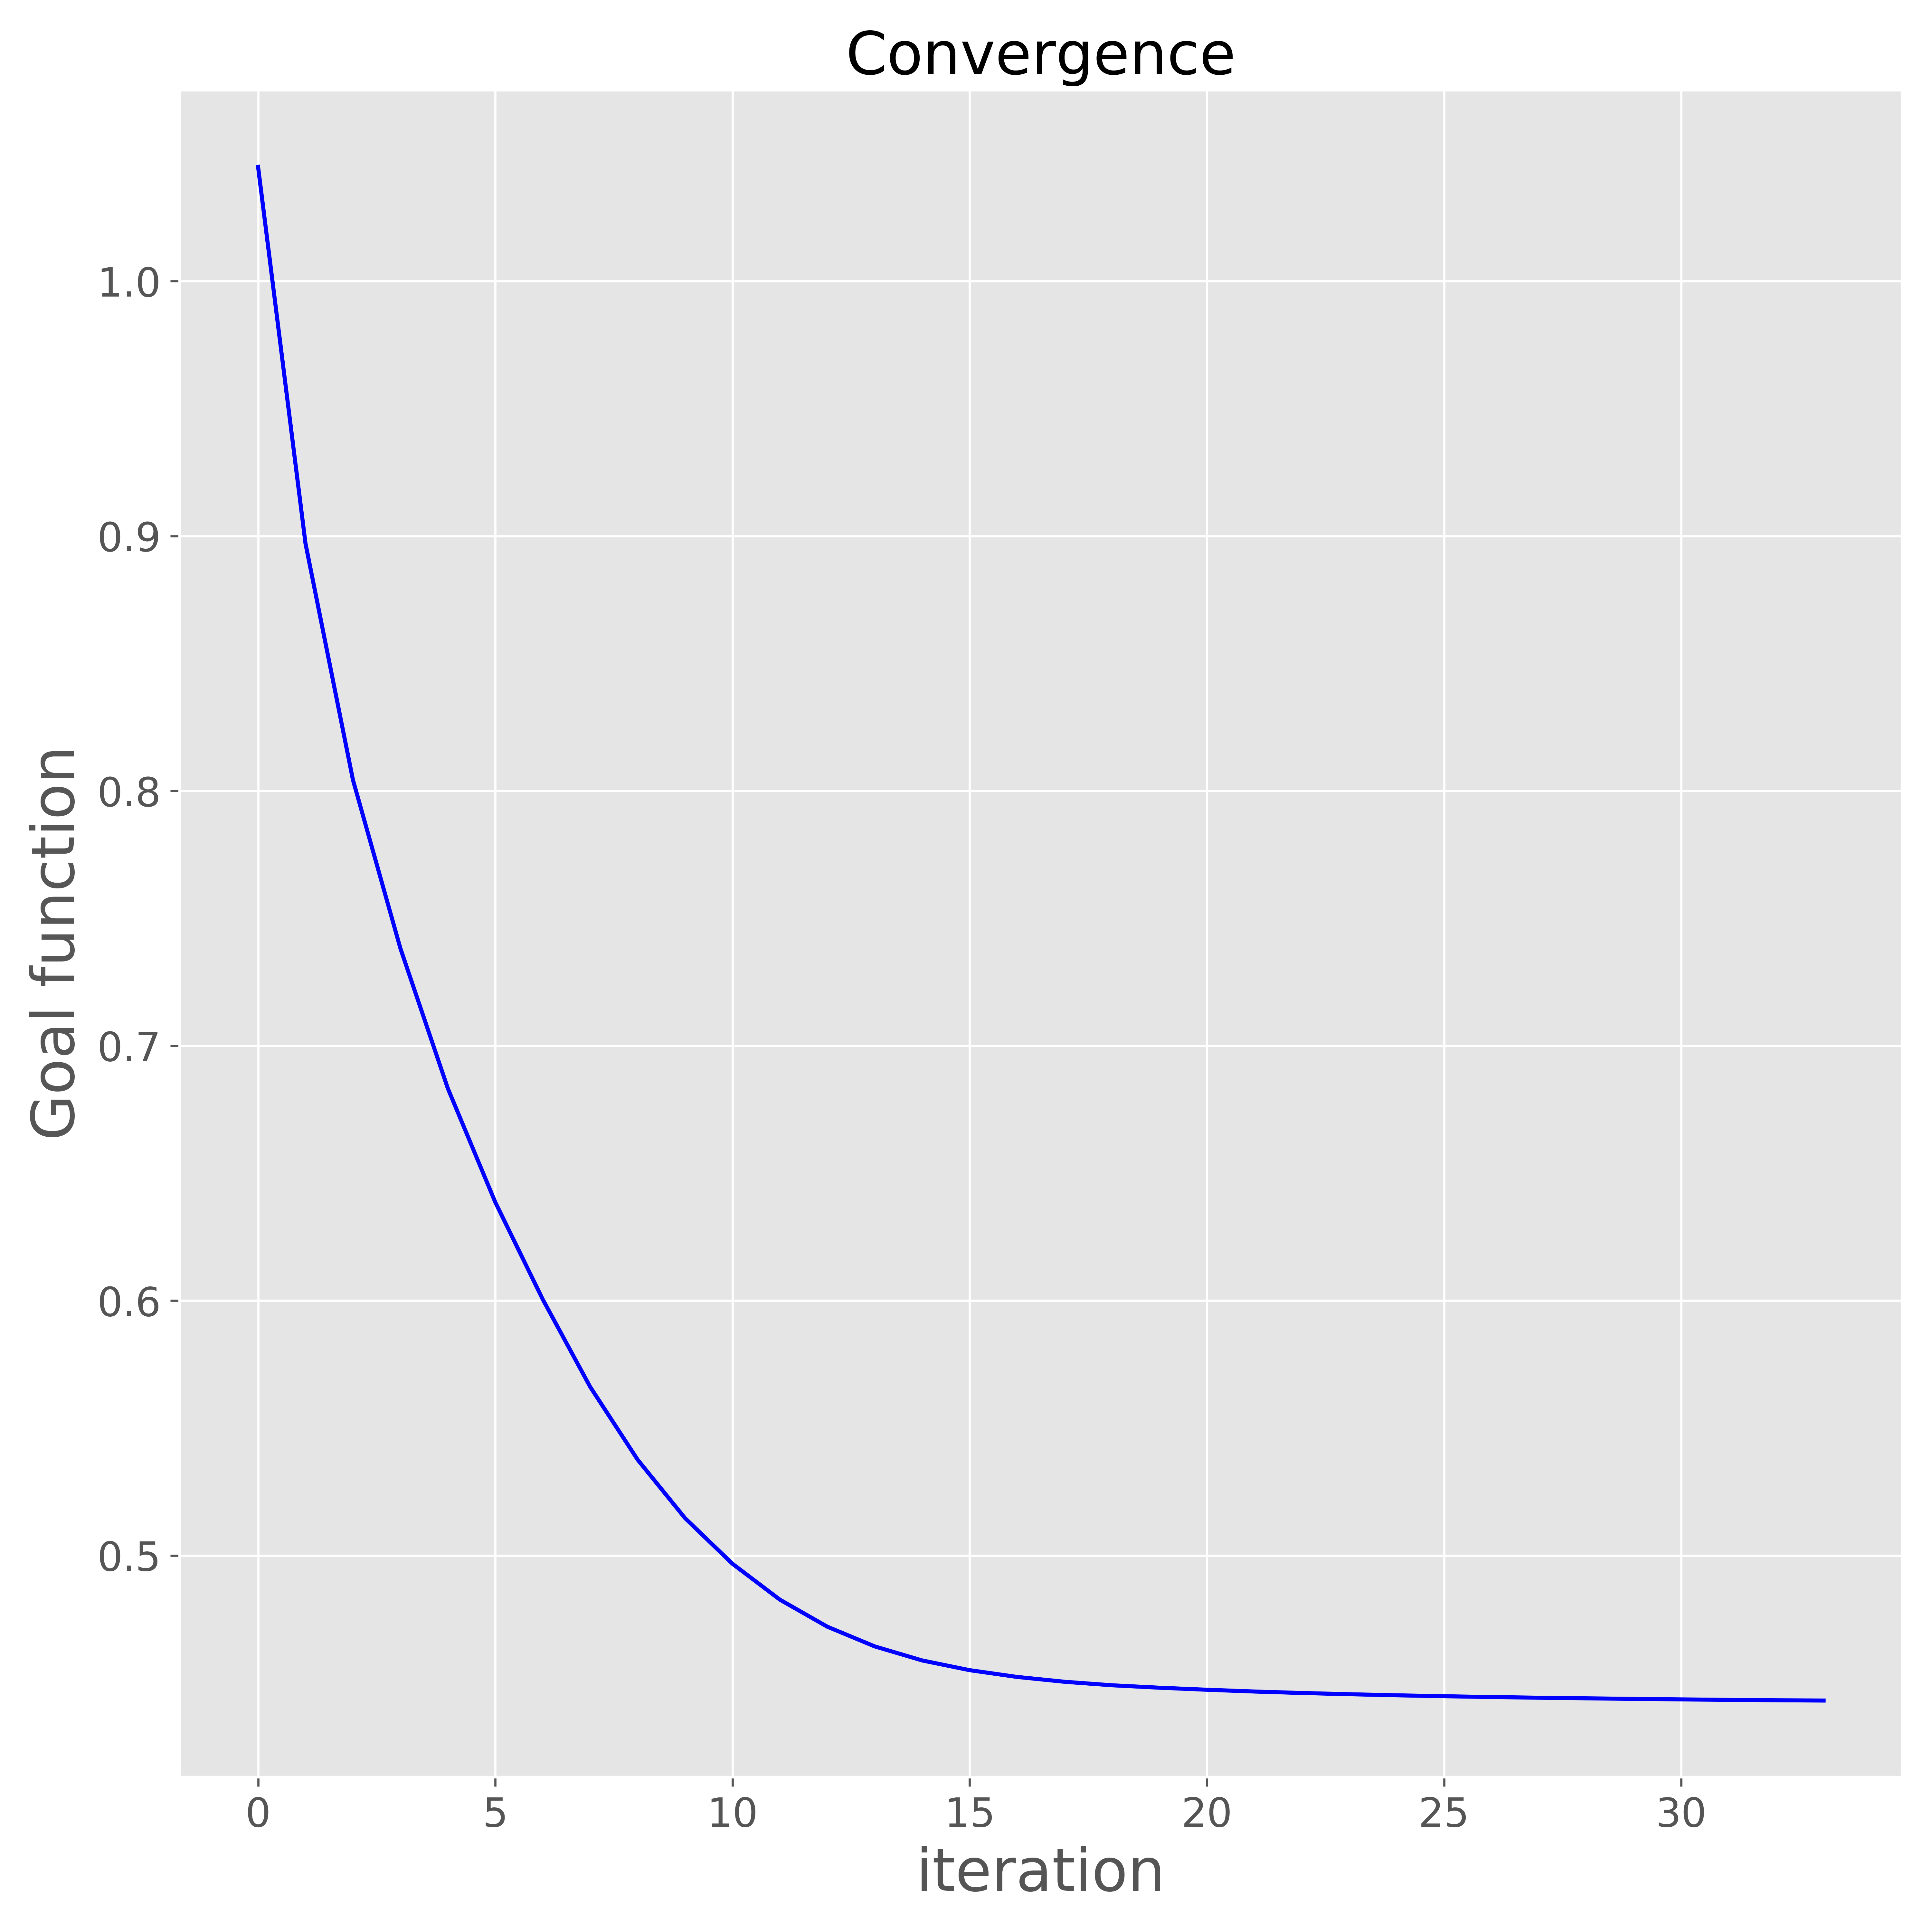
\includegraphics[width=.9\textwidth]{Fig/eqlayer/unidir_shallow_diff_test/convergence_LM_NNLS_magRM.png}
	\caption{Valor da função objetivo ao longo das iterações (equação \ref{eq:positivity_goal_function}a) mostrando a convergência do algoritmo.}
	\label{fig:convergence_3}
\end{figure}

